\usepackage{graphicx}
\usepackage{pgfpages}
\usepackage{hyperref}
\usepackage{xcolor}
\definecolor{Red}{rgb}{255, 0, 0}
\definecolor{Green}{rgb}{0, 255, 0}
\definecolor{Blue}{rgb}{0, 0, 255}
\definecolor{Cyan}{rgb}{0, 255, 255}
\definecolor{Magenta}{rgb}{255, 0, 255}
\definecolor{Yellow}{rgb}{255, 255, 0}
\definecolor{Black}{rgb}{0, 0, 0}
\definecolor{White}{rgb}{255, 255, 255}
\definecolor{lightblue}{rgb}{0.5, 0.7, 1}
\definecolor{mint}{rgb}{189, 252, 201}
\definecolor{lightmint}{rgb}{223, 255, 228}
\definecolor{mintgreen}{rgb}{152, 255, 152}
\usetheme{metropolis}
\setbeamertemplate{background canvas}[vertical shading][top=white,bottom=blue!20]
\setbeamertemplate{navigation symbols}{}
\setbeamertemplate{footline}{%
  \begin{beamercolorbox}[wd=\paperwidth,ht=2.5ex,dp=1ex,right]{footline}%
    Page \insertframenumber{} / \inserttotalframenumber
  \end{beamercolorbox}%
}
\newcommand{\frametitleimage}{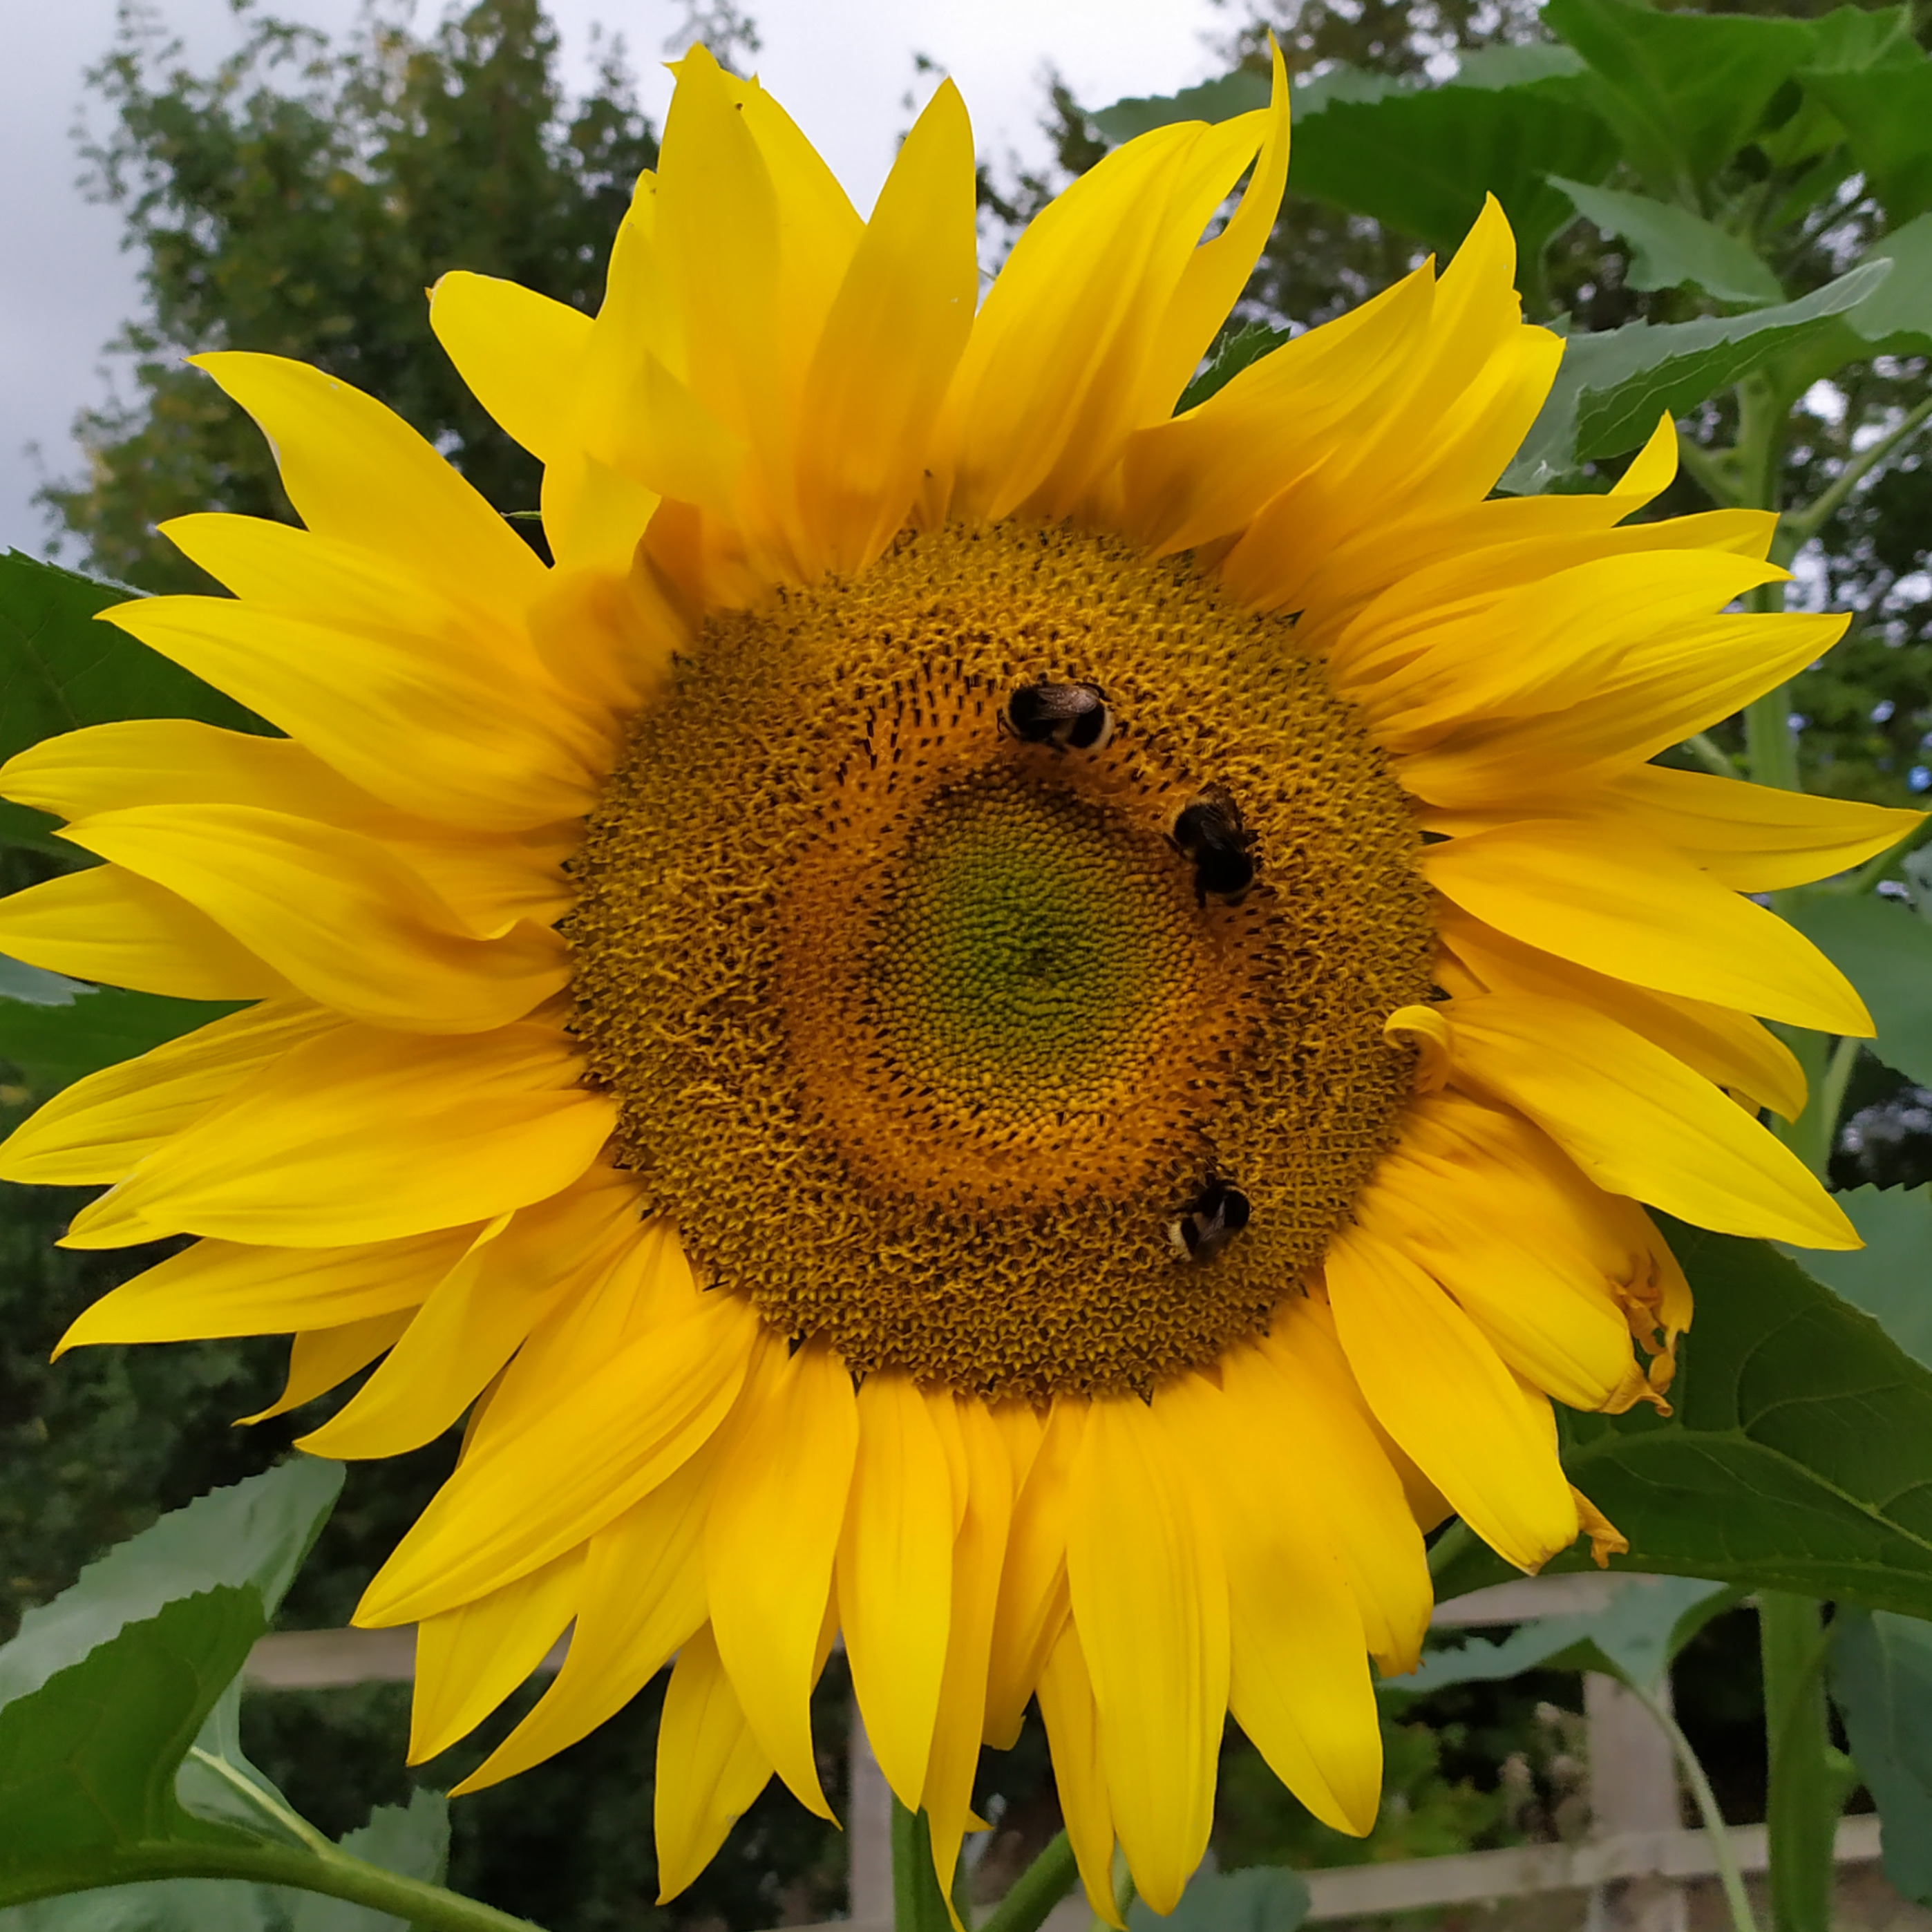
\includegraphics[height=0.7cm]{sunflower.jpg}}
\setbeamertemplate{frametitle}{%
  \pdfbookmark[1]{\insertframenumber. \insertframetitle}{frame:\insertframenumber}
  \begin{beamercolorbox}[wd=\paperwidth,ht=0.7cm,dp=1ex]{frametitle}
    \hspace*{0.5em}
    \raisebox{-0.1cm}{\frametitleimage}\vspace{-0.5cm}
    \usebeamerfont{frametitle}\insertframetitle\par
    \hfill
  \end{beamercolorbox}%
}
\transdissolve
\AtBeginDocument{
  \pdfbookmark[1]{Title Page}{titlepage}
}
\AtBeginSection[]{
  \begin{frame}
    \transdissolve
    \pdfbookmark[1]{\insertsection}{section:\insertsection}
    \frametitle{\insertsection}
    \vspace{0.5cm}
  \end{frame}
}
\newcommand{\shortframetitle}[1]{
  \gdef\insertshortframetitle{#1}
}
